\documentclass[final]{beamer}\usepackage[]{graphicx}\usepackage[]{color}
%% maxwidth is the original width if it is less than linewidth
%% otherwise use linewidth (to make sure the graphics do not exceed the margin)
\makeatletter
\def\maxwidth{ %
  \ifdim\Gin@nat@width>\linewidth
    \linewidth
  \else
    \Gin@nat@width
  \fi
}
\makeatother

\definecolor{fgcolor}{rgb}{0.345, 0.345, 0.345}
\newcommand{\hlnum}[1]{\textcolor[rgb]{0.686,0.059,0.569}{#1}}%
\newcommand{\hlstr}[1]{\textcolor[rgb]{0.192,0.494,0.8}{#1}}%
\newcommand{\hlcom}[1]{\textcolor[rgb]{0.678,0.584,0.686}{\textit{#1}}}%
\newcommand{\hlopt}[1]{\textcolor[rgb]{0,0,0}{#1}}%
\newcommand{\hlstd}[1]{\textcolor[rgb]{0.345,0.345,0.345}{#1}}%
\newcommand{\hlkwa}[1]{\textcolor[rgb]{0.161,0.373,0.58}{\textbf{#1}}}%
\newcommand{\hlkwb}[1]{\textcolor[rgb]{0.69,0.353,0.396}{#1}}%
\newcommand{\hlkwc}[1]{\textcolor[rgb]{0.333,0.667,0.333}{#1}}%
\newcommand{\hlkwd}[1]{\textcolor[rgb]{0.737,0.353,0.396}{\textbf{#1}}}%

\usepackage{framed}
\makeatletter
\newenvironment{kframe}{%
 \def\at@end@of@kframe{}%
 \ifinner\ifhmode%
  \def\at@end@of@kframe{\end{minipage}}%
  \begin{minipage}{\columnwidth}%
 \fi\fi%
 \def\FrameCommand##1{\hskip\@totalleftmargin \hskip-\fboxsep
 \colorbox{shadecolor}{##1}\hskip-\fboxsep
     % There is no \\@totalrightmargin, so:
     \hskip-\linewidth \hskip-\@totalleftmargin \hskip\columnwidth}%
 \MakeFramed {\advance\hsize-\width
   \@totalleftmargin\z@ \linewidth\hsize
   \@setminipage}}%
 {\par\unskip\endMakeFramed%
 \at@end@of@kframe}
\makeatother

\definecolor{shadecolor}{rgb}{.97, .97, .97}
\definecolor{messagecolor}{rgb}{0, 0, 0}
\definecolor{warningcolor}{rgb}{1, 0, 1}
\definecolor{errorcolor}{rgb}{1, 0, 0}
\newenvironment{knitrout}{}{} % an empty environment to be redefined in TeX

\usepackage{alltt}
\usefonttheme{serif}
\mode<presentation>{\usetheme{ASU}}
\usepackage{amsmath, amsfonts, amssymb, pxfonts, eulervm, xspace, enumerate, hyperref, color, bookmark}
\usepackage{graphicx}
\usepackage[orientation=landscape, size=a0, scale=1.4, debug]{beamerposter}
% \usepackage{natbib}

\usecolortheme{rose}
%\setbeamercolor{background canvas}{bg=magenta!16!yellow!90}

%\beamertemplategridbackground[1cm]

%-- Header and footer information ----------------------------------
\newcommand{\footright}{\href{https://github.com/STAT-ATA-ASU/Clarke-Megan}{https://github.com/STAT-ATA-ASU/Clarke-Megan}}
\newcommand{\footleft}{\href{mailto:arnholtat@appstate.edu}{Faculty Advisor: Alan Arnholt}}

\def\conference{STT 5811: Passion Driven Statistics Poster Presentation}
\title{The Association Between Low Economic Status and Access to Healthcare and the Efficacy of these on General Health}
\author{Megan Clarke} 
\institute{Department of Mathematical Sciences}
%-------------------------------------------------------------------


%-- Main Document --------------------------------------------------
\IfFileExists{upquote.sty}{\usepackage{upquote}}{}
\begin{document}
\begin{frame}[fragile]
\vspace{-2ex}
\begin{columns}[t]



%-- Column 1 ---------------------------------------------------
\begin{column}{0.31\linewidth}
\begin{minipage}[t][.955\textheight]{\linewidth} 
%-- Block 1-1
% \vspace{0ex}
\begin{block}{Introduction}
\begin{itemize}
\item Health insurance is often provided by the government if an individual does not get it through the employer or a private insurance company \cite{sommers_bd_changes_2015}.  
\item Medicaid is difficult to obtain and even those who qualify have difficulty applying and being granted assistance \cite{gaskin_economic_2012}. 
\item The Affordable Care Act (ACA) was enacted to broaden access to health insurance to improve the health of United States citizens.  
\item The purpose of this study is to examine the association between low economic status and health in subjects who do not have health insurance. 
\end{itemize}
\vspace{0ex}
\end{block}
\vfill

%-- Block 1-2
\begin{block}{Hypothesis}
\begin{itemize}
\item Null Hypothesis: There is no difference in health status of uninsured people who are unemployed and those living below the poverty line ($\leq$ 15,000/year).
\item $H_{0}$: $\mu_{unemployed}$ = $\mu_{belowpovertyline}$
\vspace{2ex}
\item Alternative Hypothesis: There is a difference in health status of uninsured people who are unemployed and those living below the poverty line.
\item $H_{A}$: $\mu_{unemployed}$ $\ne$ $\mu_{belowpovertyline}$
\end{itemize}
\vspace{0ex}
\vfill
\end{block}
\vfill

%-- Block 1-3
\begin{block}{Methods}
\begin{itemize}
\item Sample: Data collected from the National Longitudinal Study of Adolescent to Adult Health (AddHealth) Wave IV. Participants were 24 to 32 years old at the time of the study.
\item Procedure: Subjects were surveyed in the form of questionnaires using computer-assisted personal interviews (CAPI) and computer-assisted self interviews (CASI).
\item Measures: Questions from Wave I that were still applicable to young adults were repeated in Wave IV. New questions were asked pertaining to health, economics, and personal and professional stressors.
\item Implications: The ACA has caused controversy throughout the United State about the necessity of the government interfering in the healthcare field to this extent. The current study may verify the need for the ACA if low economic status limits access to healthcare and diminishes overall health.
\end{itemize}
\vspace{0ex}
\vfill
\end{block}
\vfill


\end{minipage}
\end{column}%1

%-- Column 2 ---------------------------------------------------

\begin{column}{0.31\linewidth}
\begin{minipage}[t][.955\textheight]{\linewidth} 

%-- Block 2-1
\begin{block}{Multivariate Graph}
%\vspace{0ex}


\begin{knitrout}
\definecolor{shadecolor}{rgb}{0.969, 0.969, 0.969}\color{fgcolor}

{\centering 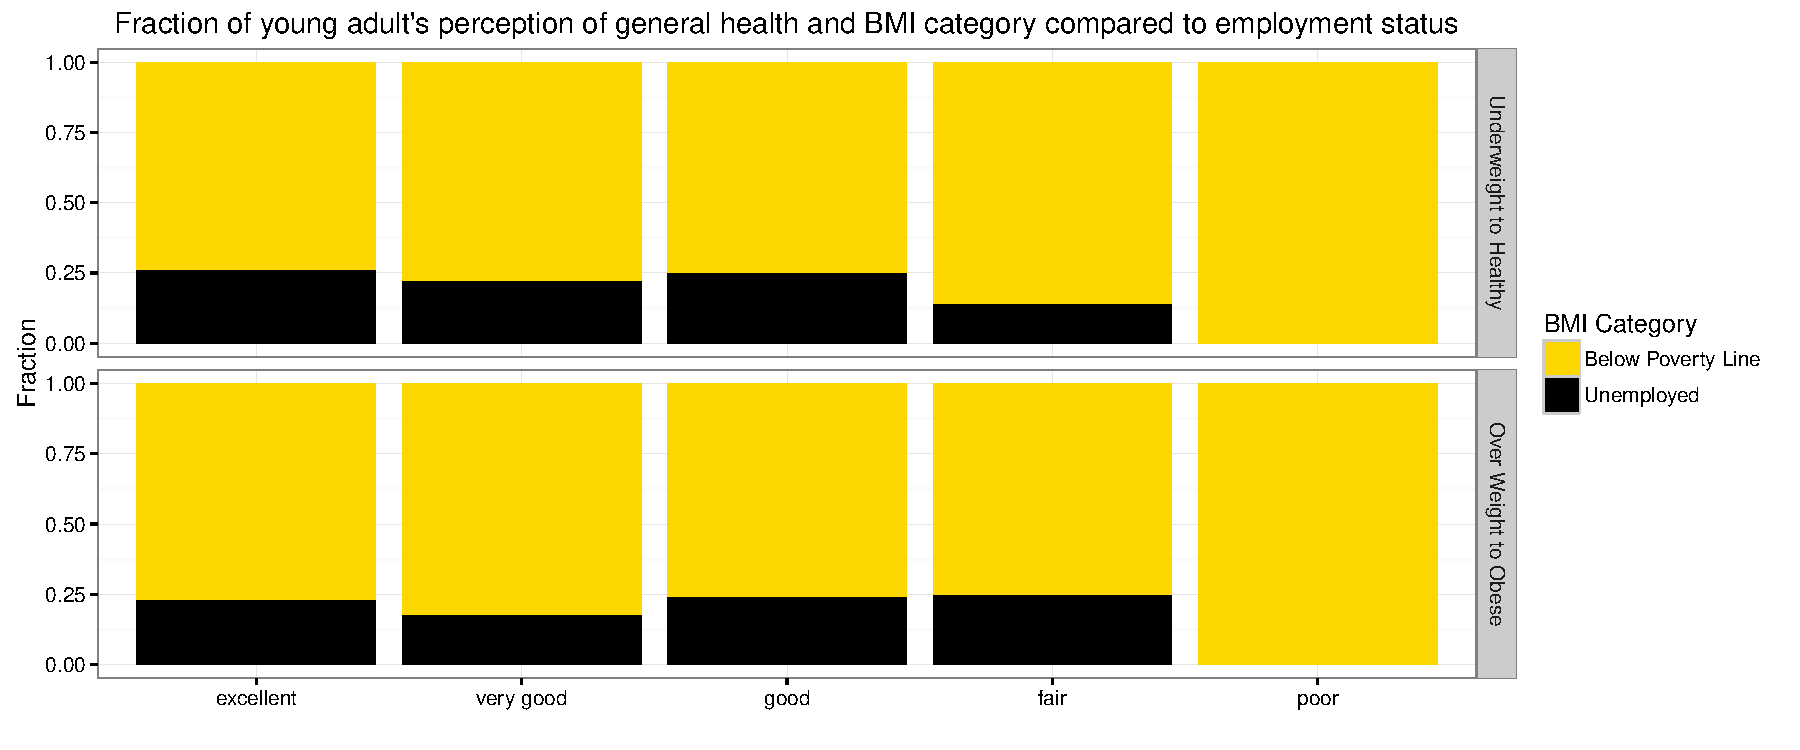
\includegraphics[width=\maxwidth]{figure/MulitvariateGraph-1} 

}



\end{knitrout}

This graph shows the general health of people without health insurance based on income. Note that all people who reported poor general health were living below the poverty line.

\vspace{-1ex}
\end{block}
\vfill

%-- Block 2-2
%\vspace{3ex}
\begin{block}{Comparing Quantitative Variables}
\vspace{0ex}

\begin{knitrout}
\definecolor{shadecolor}{rgb}{0.969, 0.969, 0.969}\color{fgcolor}

{\centering 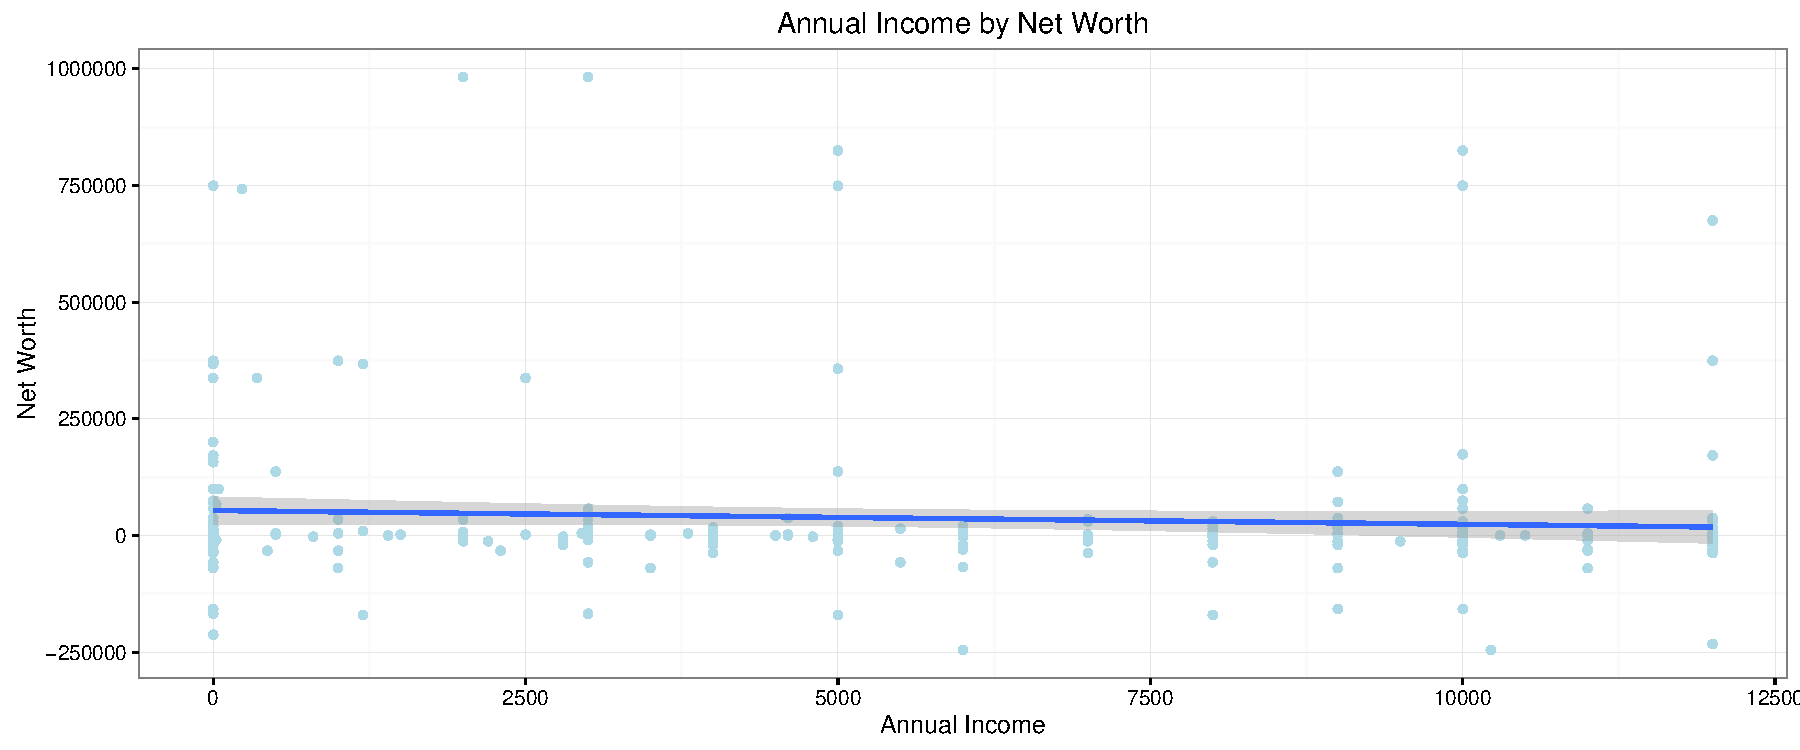
\includegraphics[width=\maxwidth]{figure/LineGraph-1} 

}



\end{knitrout}

Young people who do not have health insurance and who are at or below the poverty line often do not have a savings account or assets to have a positive net worth. As shown in this graph, many people are breaking even financially each month and do not have extra income to put towards health insurance.

\vspace{-1ex}
\end{block}
\vfill

%-- Block 2-3
%\vspace{3ex}
\begin{block}{Violin Graph}
\vspace{0ex}
\begin{knitrout}
\definecolor{shadecolor}{rgb}{0.969, 0.969, 0.969}\color{fgcolor}

{\centering 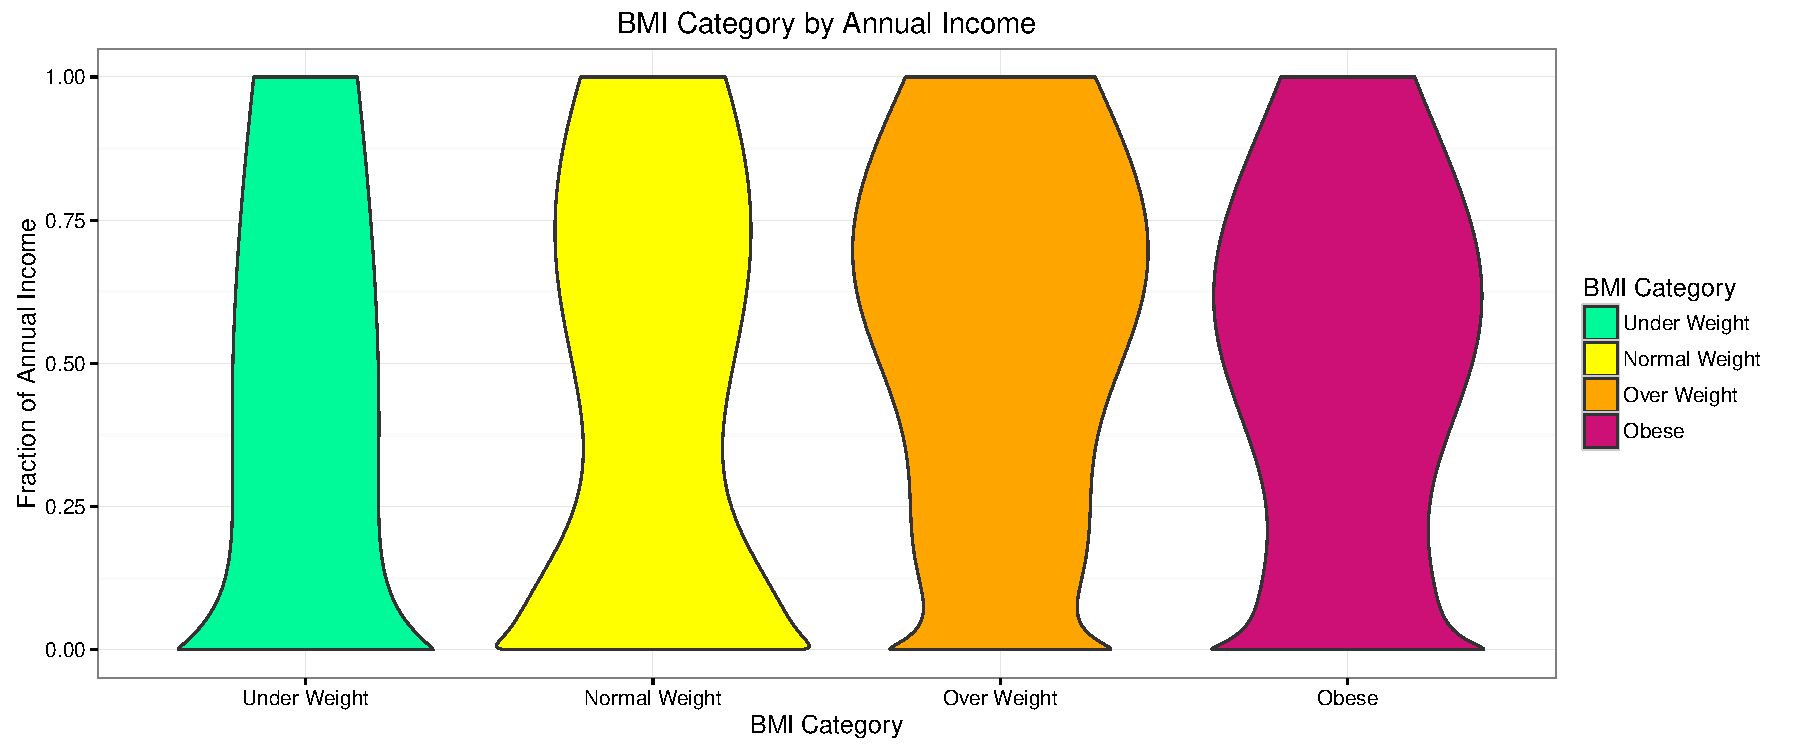
\includegraphics[width=\maxwidth]{figure/ViolinGraphs-1} 

}



\end{knitrout}

This violin graph illustrates the BMI category of people with a certain income. There are more people overweight and obese who have incomes closer to the poverty line.

\vspace{-1ex}
\end{block}
\vfill

\end{minipage}
\end{column}%2

%-- Column 3 ---------------------------------------------------
\begin{column}{0.31\linewidth}
\begin{minipage}[t][.955\textheight]{\linewidth} 
%-- Block 3-1
\vspace{0ex}
\begin{block}{Results}
\vspace{0ex}
\begin{itemize}
\item There were statistically significant differences between unemployed and those living below the poverty line who had a positive net worth and those who had zero net worth. 
\item Significant differences were also shown between those who reported poor general health and those who reported excellent.
\item However, in young people aged 24 to 32, there were no differences between general health
and employment status. 
\end{itemize}
\vspace{1ex}
\vfill
\end{block}
\vfill

%-- Block 3-2
\begin{block}{Discussion}
\begin{itemize}
\item Since there were differences between the poor and excellent general health categories, it is an indication that there is validity to this scale. 
\item There are not differences between the BMI categories and health perception categories, which shows that BMI is an adequate quantitative assessment of general health.
\item Within this age category (ages 24 to 32), there are not enough differences in low income to unemployed individuals to assess the differences between income and general health in individuals without access to healthcare. 
\end{itemize}
\vspace{0ex}
\vfill
\end{block}
\vfill

%-- Block 3-3
\vspace{0ex}
\begin{block}{Further Direction}
\vspace{0ex}
\begin{itemize}
\item Use a broader age range or use older individuals who may be experiencing more health related issues
\item Compare participants with and without health insurance to determine differences in health even below the poverty line
\item A future study could use a different measurement other than self perception of health or BMI. These have been shown to not be particularly accurate measurements, but are commonly used to assess a large group of subjects from the general population.
\end{itemize}
\vspace{1ex}
\vfill
\end{block}
\vfill

%-- Block 3-4
\begin{block}{References}
\footnotesize
\setbeamertemplate{bibliography item}[text]
\vspace{-1ex}


\bibliographystyle{plain}  % can use plain but comment out natbib at top if using plain
\bibliography{knitr-packages,ResearchPDS}
\normalsize
\vfill
\end{block} 
\vfill

\end{minipage}
\end{column}%3




\end{columns}
\end{frame}
\end{document}
